\documentclass[../main.tex]{subfiles}

\begin{document}
\section{Reverse challenges}

\subsection{Breach}
With the "Breach" challenge, it is the goal to hack the elections in the Florida. 

The programmers of Florida made an application so that the authorized employees could generate a code to bring the voting letters to the vault, from where the voting letters will be counted.

Maybe if we are a bit sneaky, we can manipulate the voting system. After having hacked into an employee's laptop, we were able to recover a deleted file. Too bad it was damaged, find out if you can restore the program and get the passwords. Let's make America great again, together.

\subsubsection{Challenge explained}

For this challenge, you will receive an ELF or a disassembly file. The app itself will be hosted on our servers.

The app is written in C language and consists of 4 functions

Function 1: secret\_door(), this function will ask for a PIN code to open the door.\\
Function 2: big\_vault(), this function will ask for a password and the string will be flipped.\\
Function 3: hack\_the\_election(), this function reads the flag from a txt file and returns it.\\
Function 4: check() this will check if the first 2 functions have been executed correctly. Once this is done, it will call the 3rd function.

The participant will have to analyse the ELF file and preferably open it in one of the disassembly tools. This way he will be able to find out what the PIN is and he will have to investigate the function of big\_vault to understand that the password is stored as a reverse string. 

The app can be found on GitHub.

\subsubsection{Write up}

There are several ways to solve this challenge, the main one is that you only see the flag when the app is hosted.

The best way is to use a reverse tool so you can see which passwords you need and how to get them. 


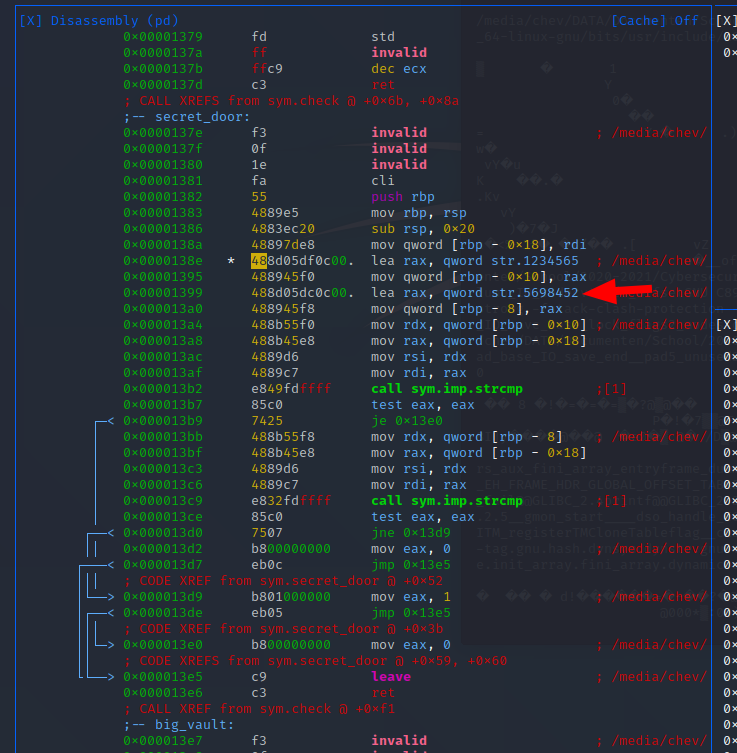
\includegraphics[width=\linewidth]{images/Nicolai/lab_assembly_pin1.png}

Here you can find the first PIN

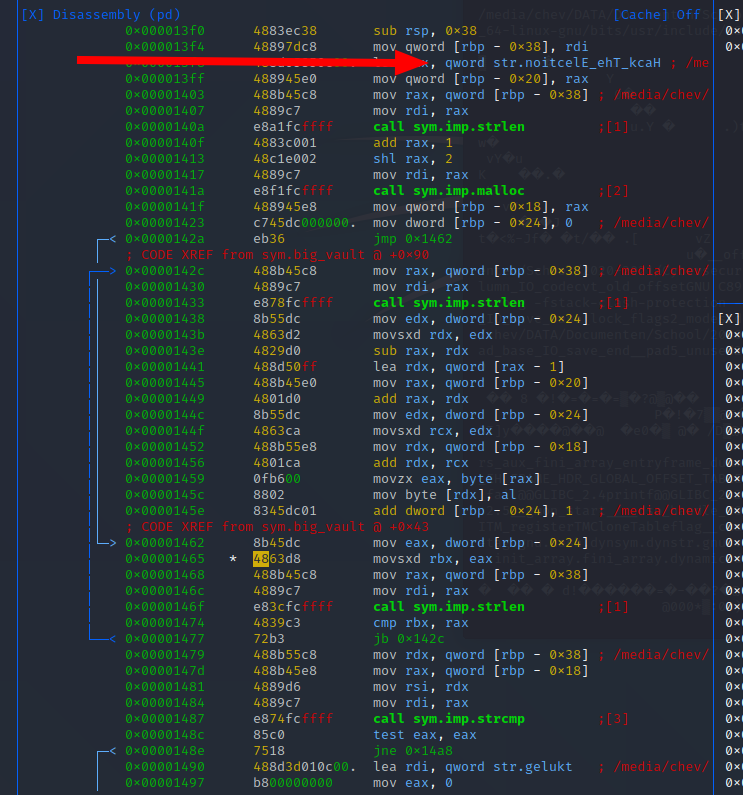
\includegraphics[width=\linewidth]{images/Nicolai/lab_assembly_pin2.png}
Here we notice a strange string, after good analysis we notice that it is a reverse string

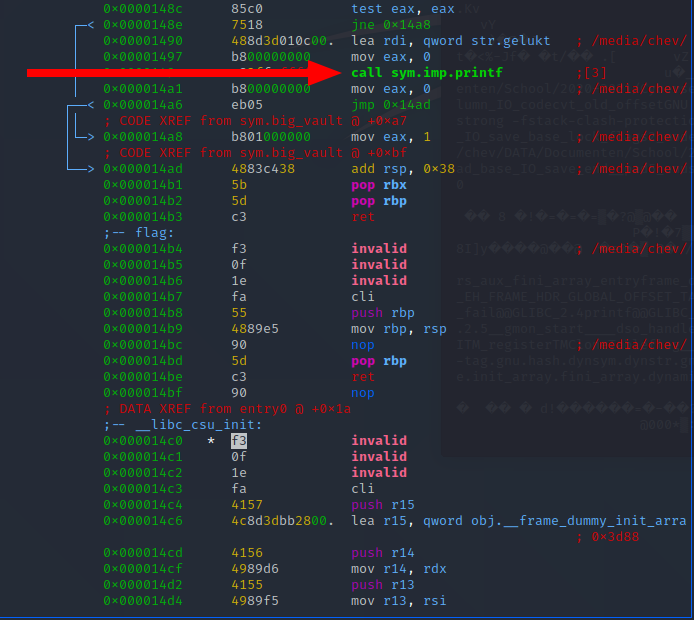
\includegraphics[width=\linewidth]{images/Nicolai/lab_assembly_print.png}

\end{document}